\documentclass[tikz]{standalone}
\usepackage[utf8]{inputenc}
\usepackage{amsmath}
\usetikzlibrary{intersections}

\begin{document}

% unit circle and node
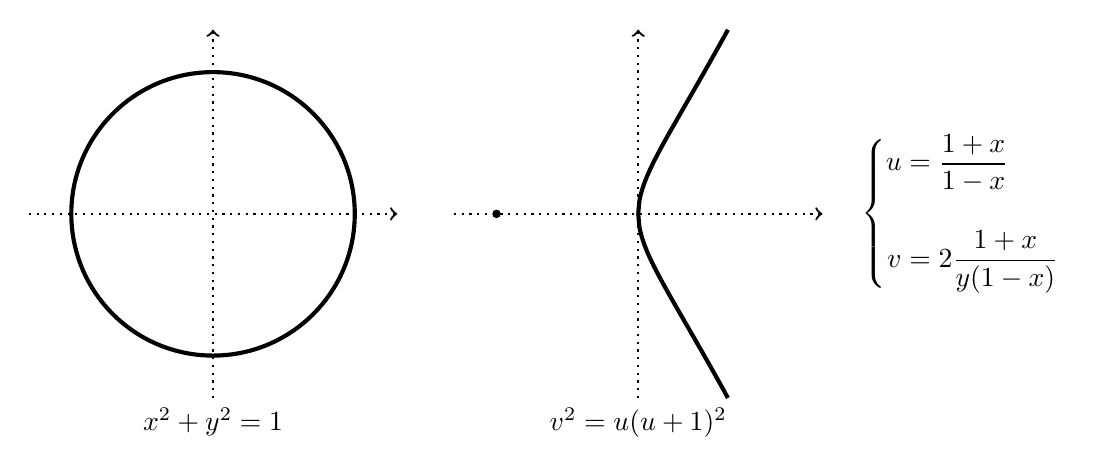
\begin{tikzpicture}[thick,scale=1.8]
\def\ptsize{.03}
\draw[->,dotted] (-1.3, 0) -- (1.3,0);
\draw[->,dotted] (0,-1.3) -- (0,1.3);
\coordinate (inf) at (1,0);
\path[draw,name path=circ,line width=1.5pt] (0,0) circle (1);
\node[below] at (0,-1.3) {$x^2 + y^2 = 1$};

\begin{scope}[shift={(3,0)}]
\draw[->,dotted] (-1.3, 0) -- (1.3,0);
\draw[->,dotted] (0,-1.3) -- (0,1.3);
\fill (-1,0) circle (\ptsize);
\draw[domain=0:.633,smooth,samples=80,line width=1.5pt] plot (\x, {sqrt(\x*(\x + 1)^2)});
\draw[domain=0:.633,smooth,samples=80,line width=1.5pt] plot (\x, {-sqrt(\x*(\x + 1)^2)});
\node[below] at (0,-1.3) {$v^2 = u(u+1)^2$};
\node[right] at (1.5,0) {\hbox{$\left\{\begin{aligned}u &= \frac{1+x}{1-x} \\[10pt] v&=2\frac{1+x}{y(1-x)}\end{aligned}\right.$}};
\end{scope}
    
\end{tikzpicture}

\end{document}